\documentclass{standalone}
\usepackage{tikz}
\usepackage{ctex,siunitx}
\usepackage{tkz-euclide}
\usepackage{amsmath}
\usetikzlibrary{patterns, calc}
\usetikzlibrary {decorations.pathmorphing, decorations.pathreplacing, decorations.shapes}
\tikzset{
  boat/.pic={
    \fill[line join=round,gray,draw](-0.1,-0.1)--(0.1,-0.1)[bend right=30]to(0,0.4)[bend right=30]to cycle;
    \fill[line join=round,darkgray,draw](-0.08,0)--(0.08,0)[bend right=20]to(0,0.32)[bend right=20]to cycle;
  }
}
\begin{document}
\small
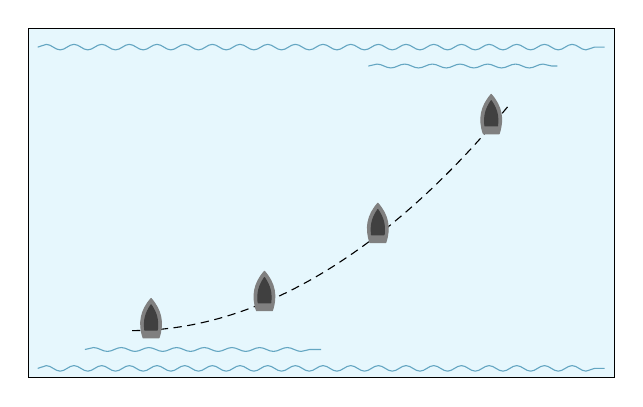
\begin{tikzpicture}[>=stealth,scale=1.2]
  % \useasboundingbox (-0.1,0.1) rectangle(6.1,-3.1);
  \draw[fill=cyan!10](-1.1,-0.5) rectangle(5.1,3.2);
  \draw[decorate,decoration={snake,amplitude=1pt}, gray!50!cyan](-1,3)--(5,3);
  \draw[decorate,decoration={snake,amplitude=1pt}, gray!50!cyan](-1,-0.4)--(5,-0.4);
  \draw[decorate,decoration={snake,amplitude=.7pt},gray!50!cyan](2.5,2.8)--(4.5,2.8);
  \draw[decorate,decoration={snake,amplitude=.7pt},gray!50!cyan](-0.5,-0.2)--(2.0,-0.2);
  \draw[densely dashed](0,0) parabola (4,2.4);
  \foreach \x in { 0.2,1.4,2.6,3.8 } {\pic at (\x,0.15*\x*\x) {boat};}
\end{tikzpicture}
\end{document}